\documentclass[aspectratio=169]{../latex_main/tntbeamer}  % you can pass all options of the beamer class, e.g., 'handout' or 'aspectratio=43'
\usepackage{dsfont}
\usepackage{bm}
\usepackage[english]{babel}
\usepackage[T1]{fontenc}
%\usepackage[utf8]{inputenc}
\usepackage{graphicx}
\graphicspath{ {./figures/} }
\usepackage{algorithm}
\usepackage[ruled,vlined,algo2e,linesnumbered]{algorithm2e}
\usepackage{hyperref}
\usepackage{booktabs}
\usepackage{mathtools}

\usepackage{amsmath,amssymb}

\DeclareMathOperator*{\argmax}{arg\,max}
\DeclareMathOperator*{\argmin}{arg\,min}

\usepackage{amsbsy}
\newcommand{\vect}[1]{\bm{#1}}
%\newcommand{\vect}[1]{\boldsymbol{#1}}

\usepackage{pgfplots}
\pgfplotsset{compat=1.16}
\usepackage{tikz}
\usetikzlibrary{trees} 
\usetikzlibrary{shapes.geometric}
\usetikzlibrary{positioning,shapes,shadows,arrows,calc,mindmap}
\usetikzlibrary{positioning,fadings,through}
\usetikzlibrary{decorations.pathreplacing}
\usetikzlibrary{intersections}
\pgfdeclarelayer{background}
\pgfdeclarelayer{foreground}
\pgfsetlayers{background,main,foreground}
\tikzstyle{activity}=[rectangle, draw=black, rounded corners, text centered, text width=8em]
\tikzstyle{data}=[rectangle, draw=black, text centered, text width=8em]
\tikzstyle{myarrow}=[->, thick, draw=black]

% Define the layers to draw the diagram
\pgfdeclarelayer{background}
\pgfdeclarelayer{foreground}
\pgfsetlayers{background,main,foreground}

% Requires XeLaTeX or LuaLaTeX
%\usepackage{unicode-math}

\usepackage{fontspec}
%\setsansfont{Arial}
\setsansfont{RotisSansSerifStd}[ 
Path=../latex_main/fonts/,
Extension = .otf,
UprightFont = *-Regular,  % or *-Light
BoldFont = *-ExtraBold,  % or *-Bold
ItalicFont = *-Italic
]
\setmonofont{Cascadia Mono}[
Scale=0.8
]

% scale factor adapted; mathrm font added (Benjamin Spitschan @TNT, 2021-06-01)
%\setmathfont[Scale=1.05]{Libertinus Math}
%\setmathrm[Scale=1.05]{Libertinus Math}

% other available math fonts are (not exhaustive)
% Latin Modern Math
% XITS Math
% Libertinus Math
% Asana Math
% Fira Math
% TeX Gyre Pagella Math
% TeX Gyre Bonum Math
% TeX Gyre Schola Math
% TeX Gyre Termes Math

% Literature References
\newcommand{\lit}[2]{\href{#2}{\footnotesize\color{black!60}[#1]}}

%%% Beamer Customization
%----------------------------------------------------------------------
% (Don't) Show sections in frame header. Options: 'sections', 'sections light', empty
\setbeamertemplate{headline}{empty}

% Add header logo for normal frames
\setheaderimage{
	% 
\includegraphics[height=\logoheight]{figures/TNT_darkv4.pdf}
	
\includegraphics[height=\logoheight]{../latex_main/figures/luh_logo_rgb_0_80_155.pdf}
	% 
\includegraphics[height=\logoheight]{figures/logo_tntluh.pdf}
}

% Header logo for title page
\settitleheaderimage{
	% 
\includegraphics[height=\logoheight]{figures/TNT_darkv4.pdf}
	
\includegraphics[height=\logoheight]{../latex_main/figures/luh_logo_rgb_0_80_155.pdf}
	% 
\includegraphics[height=\logoheight]{figures/logo_tntluh.pdf}
}

% Title page: tntdefault 
\setbeamertemplate{title page}[tntdefault]  % or luhstyle
% Add optional title image here
%\addtitlepageimagedefault{
\includegraphics[width=0.65\textwidth]{figures/luh_default_presentation_title_image.jpg}}

% Title page: luhstyle
% \setbeamertemplate{title page}[luhstyle]
% % Add optional title image here
% \addtitlepageimage{
\includegraphics[width=0.75\textwidth]{figures/luh_default_presentation_title_image.jpg}}

\author[Abedjan \& Lindauer]{Ziawasch Abedjan \& Marius Lindauer\\[1em]
	
\includegraphics[height=\logoheight]{../latex_main/figures/luh_logo_rgb_0_80_155.pdf}\qquad
	
\includegraphics[height=\logoheight]{../latex_main/figures/DBIS_Kurzlogo.png}\qquad

\includegraphics[height=\logoheight]{../latex_main/figures/TNT_darkv4}\qquad

\includegraphics[height=\logoheight]{../latex_main/figures/L3S.jpg}	}
\date{Summer Term 2022; \hspace{0.5em} {
\includegraphics[height=1.5em]{../latex_main/figures/Cc-by-nc-sa_icon.svg.png}}; based on \href{https://ds100.org/fa21/}{[DS100]}
}


%%% Custom Packages
%----------------------------------------------------------------------
% Create dummy content
\usepackage{blindtext}

% Adds a frame with the current page layout. Just call \layout inside of a frame.
\usepackage{layout}


%%% Macros
%\renewcommand{\vec}[1]{\mathbf{#1}}
% \usepackage{bm}
%\let\vecb\bm

\title[Introduction]{DS: Introduction to Modeling}
\subtitle{Minimizing mean squared error (MSE)}

\graphicspath{ {./figure/} }
%\institute{}


\begin{document}
	
	\maketitle
	\begin{frame}{Minimizing MSE}
	    We saw with the toy example of [20, 21, 22, 29, 33] that the value that minimizes the MSE of the constant model was 25, which was the mean of our observations.\\
	    \bigskip
	    We can try other examples if we want to, and we’ll end up with the same result. Let’s instead pivot to proving this rigorously, using mathematics. There are two ways we’ll go about doing this:
	    \begin{itemize}
	        \item Using calculus.
	        \item Using a neat algebraic trick.
	    \end{itemize}
	    \bigskip
	    For both derivations, the slides contain the key ideas, but the lecture videos will contain a step-by-step walkthrough.
	\end{frame}
	
	
	\begin{frame}{MSE minimization using calculus}
	    One way to minimize a function is by using calculus: we can take the derivative, set it equal to 0, and solve for the optimizing value.
	    \begin{itemize}
	        \item The derivative of the sum of several pieces is equal to the sum of the derivative of said pieces.
	        \item The derivative of the loss for a single point is    $\frac{d}{d\theta} (y_i - \theta)^2 = 2(y_i - \theta)(-1) = -2(y_i - \theta)$.                                
	    \end{itemize}
	    Then:\\
	    \vspace{2.5cm}
	    \hspace{6.5cm} 
\includegraphics[scale=.4]{Bild27}\\
	    \vspace{-2.5cm}
	    
	    \vspace{-.7cm}
	    \hspace{10.5cm} 
\includegraphics[scale=.4]{Bild28}\\
	    \vspace{0.7cm}
	    
	    \vspace{-3cm}
	    \begin{align*}
	        R(\theta) &= \frac{1}{n}\sum\limits_{i=1}^n(y_i - \theta)^2\\
	        \rightarrow \frac{d}{d\theta}R(\theta)  &= \frac{1}{n} \sum\limits_{i=1}^n\frac{d}{d\theta}(y_i -\theta)^2 = \frac{1}{n}\sum\limits_{i=1}^n(-2)(y_i - \theta) = \frac{-2}{n}\sum\limits_{i=1}^n(y_i - \theta)
	    \end{align*}
	\end{frame}
	
	
	
	\begin{frame}{MSE minimization using calculus}
	     %\begin{align*}
	       % R(\theta) &= \frac{1}{n}\sum\limits_{i=1}^n(y_i - \theta)^2\\
	      %  \rightarrow \frac{d}{d\theta}R(\theta)  &= \frac{1}{n} \sum\limits_{i=1}^n\frac{d}{d\theta}(y_i -\theta)^2 = \frac{1}{n}\sum\limits_{i=1}^n(-2)(y_i - \theta) = \frac{-2}{n}\sum\limits_{i=1}^n(y_i - \theta)
	   % \end{align*}
	    
	    \vspace{0.5cm}
	    \hspace{8cm} 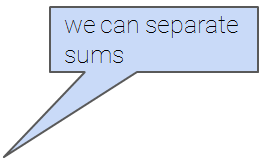
\includegraphics[scale=.4]{Bild29}\\
	    \vspace{-0.5cm}
	    
	    
	    \vspace{1cm}
	    \hspace{11cm} 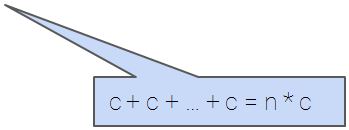
\includegraphics[scale=.4]{Bild30}\\
	    \vspace{-1cm}
	    
	    \vspace{-3.5cm}
	    Setting this term to 0, we have:
        \begin{align*}
            0 &= \frac{-2}{n}\sum\limits_{i=1}^n(y_i - \theta)\\
            0 &= \sum\limits_{i=1}^n(y_i - \theta) = \sum\limits_{i=1}^ny_i - \sum\limits_{i=1}^n\theta = \sum\limits_{i=1}^ny_i - n\theta\\
            n\theta &= \sum\limits_{i=1}^ny_i\\
            \rightarrow \hat{\theta} &= \frac{\sum_{i=1}^ny_i}{n} = mean(y)
        \end{align*}
        Thus, with squared loss and the constant model, the sample mean minimizes MSE.
	\end{frame}
	
	
	\begin{frame}{MSE minimization using calculus}
	    \vspace{-1cm}
	    \begin{equation*}
	        \rightarrow \hat{\theta} &= \frac{\sum_{i=1}^ny_i}{n} = mean(y)
	    \end{equation*}
	    We’re not done yet! To be thorough, we need to perform the second derivative test, to guarantee that the point we found is truly a minimum (rather than a maximum or saddle point). We hope that the second derivative of our objective function is positive, indicating our function is convex opening upwards.
	    \begin{align*}
	        \frac{d}{d\theta}R(\theta) &= \frac{-2}{n}\sum\limits_{i=1}^n(y_i - \theta)\\
	        \frac{d^2}{d\theta^2}R(\theta) &= \frac{-2}{n}\sum\limits_{i=1}^n(0 - 1)  = \frac{2}{n}\sum\limits_{i=1}^n1 = 2
	    \end{align*}
	    Fortunately, it is, so the sample mean truly is the minimizer we were looking for. We will interpret what this means shortly.
	\end{frame}
	
	
	\begin{frame}{MSE minimization using an algebraic trick}
	    \vspace{-.5cm}
	    It turns out that in this case, there’s another rather elegant way of performing the same minimization algebraically, but without using calculus.
	    \begin{itemize}
	        \item We present this derivation in the next few slides. The lecture video will walk through it in detail.
	        \item In this proof, you will need to use the fact that the sum of deviations from the mean is 0 (in other words, that        $\sum\limits_{i=1}^n(y_i - \overline{y}) = 0$               ). We present that proof here:\\
	            $\sum_{i=1}^n(y_i - \overline{y}) = \sum_{i=1}^ny_i - \sum_{i=1}^n\overline{y}\\
	           \hspace{2.9cm} = \sum_{i=1}^ny_i - n\overline{y} \\
	           \hspace{3cm}= \sum_{i=1}^ny_i - n\cdot \frac{1}{n} \sum_{i=1}^ny_i \\
	           \hspace{3cm}= \sum_{i=1}^ny_i - \sum_{i=1}^ny_i\\
	            \hspace{3cm}= 0$
	            
	        \item Our proof will also use the definition of the variance of a sample. As a refresher:
	        $\sigma_y^2 = \frac{1}{n}\sum_{i=1}^n(y_i - \overline{y})^2$\\
	        \vspace{-3.5cm}
	        \hspace{8cm}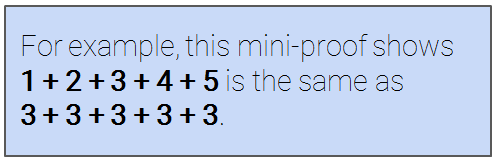
\includegraphics[scale=.5]{Bild31}\\
	        \vspace{3.5cm}
	        
	        
	        \vspace{-2.7cm}
	        \hspace{4cm}
\includegraphics[scale=.3]{Bild32}\\
	        \vspace{2.7cm}
	    \end{itemize}
	\end{frame}
	
	
	
	\begin{frame}{MSE minimization using an algebraic trick}
	    \begin{columns}
	        \begin{column}{.65\textwidth}
	                    
	                   \vspace{5.5cm}
	                   \hspace{0.1cm} 
\includegraphics[scale=.3]{Bild34}\\
	                   \vspace{-5.5cm}
	                   
	                   \vspace{-1.5cm}
	                    $R(\theta) = \dfrac{1}{n} \sum\limits_{i=1}^n(y_i - \theta)^2\\
	                    %\bigskip
	                   \hspace{1cm}= \dfrac{1}{n}  \sum_{i=1}^n[(y_i - \overline{y}) + (\overline{y} - \theta)]^2\\
	                   %\bigskip
	                   \hspace{1cm}= \dfrac{1}{n} \sum_{i=1}^n[(y_i - \overline{y})^2 + 2(y_i - \overline{y})(\overline{y} - \theta) + (\overline{y} - \theta)^2]\\
	                   %\bigskip
	                   \hspace{1cm}= \dfrac{1}{n} [\sum_{i=1}^n(y_i - \overline{y})^2 +2(\overline{y} - \theta)\sum_{i=1}^n(y_i - \overline{y}) + n(\overline{y} - \theta)^2]\\
	                   %\bigskip
	                   \hspace{1cm}= \dfrac{1}{n} \sum_{i=1}^n(y_i - \overline{y})^2 +\frac{2}{n}(\overline{y} - \theta)\cdot 0 + (\overline{y} - \theta)^2\\
	                  %\bigskip
	                   \hspace{1cm} = \sigma_y^2 + (\overline{y} - \theta)^2
	                   $\\
	                   \vspace{-1cm}
	                   \hspace{5.3cm} 
\includegraphics[scale=.3]{Bild33}\\
	                   \vspace{1cm}
	                   
	                   
	                   
	        \end{column}
	        
	        
	        \begin{column}{.35\textwidth}
	                   \\
	                   \vspace{-.5cm}
	                This proof relies on an algebraic trick. We can write the difference a - b as 
                    (a - c) + (c - b), where a, b, and c are any numbers.\\
                    \bigskip
                    Using that fact, we can write
                     $y_i - \theta = (y_i - \overline{y}) +  (\overline{y} -\theta)$, where
                    $\overline{y} = \frac{1}{n} \sum_{i=1}^ny_i $ , our sample mean.\\
                    \bigskip
                    Also note: going from line 3 to 4, we distribute the sum to the individual terms. This is a property of sums you should become familiar with!
	        \end{column}
	    \end{columns}
	\end{frame}
	
	
	
	\begin{frame}{Minimization using an algebraic trick}
	    In the previous slide, we showed that          $R(\theta) = \sigma^2_y + (\overline{y} - \theta )^2$.
	    \begin{itemize}
	        \item Since variance can’t be negative, the first term is greater than or equal to 0.
	        \begin{itemize}
	            \item Of note, the first term doesn’t involve  $\theta$   at all. Changing our model won’t change this value, so for the purposes of determining   $\hat{\theta}$   , we can ignore it.
	        \end{itemize}
	        \item The second term is being squared, and so also must be greater than or equal to 0.
	        \begin{itemize}
	            \item This term does involve    $\theta$, and so picking the right value of $\theta$     will minimize our average loss.
	            \item We need to pick the    $\theta$  that sets the second term to 0.
	            \item This is achieved when      $\theta = \overline{y}$         . In other words: 
                \begin{equation*}
                    \hat{\theta} = \overline{y} = \text{mean}(y)
                \end{equation*}
	        \end{itemize}
	    \end{itemize}
	    Looks familiar!\\
	    Question: What is the value of average loss, when evaluated at       $\theta = \hat{\theta}$        ? 
	\end{frame}
	
	
	\begin{frame}{Minimum value of MSE is the sample variance}
	    It’s worth noting that when we substitute     $\theta = \overline{y}$            back into our average loss, we obtain a familiar result:
	    \begin{equation*}
	        R(\overline{y}) = \frac{1}{n}\sum\limits_{i=1}^n(y_i - \overline{y})^2 = \sigma^2_y
	    \end{equation*}
	    \bigskip\\
	    That is, the minimum value that mean squared error can take on (again, for the constant model) is the sample variance. \\
	    \bigskip
	    Put another way, the following statement is true whenever      $\theta \neq \overline{y}$         : \\
	    \begin{equation*}
	        \frac{1}{n}\sum\limits_{i=1}^n(y_i - \overline{y})^2 < \frac{1}{n}\sum\limits_{i=1}^n(y_i - \theta)^2
	    \end{equation*}
	\end{frame}
	
	
	
	\begin{frame}{Mean minimizes MSE for the constant model}
	    As we determined a variety of ways, for the constant model with squared loss, the mean of the dataset is the optimal model.
	    \begin{equation*}
	        \hat{\theta} = \text{mean}(y) = \overline{y}
	    \end{equation*}
	    \begin{itemize}
	        \item This holds true regardless of the dataset we use, but it’s only true for this combination of model and loss.
	        \item If we choose any other constant other than the sample mean, the empirical risk will not be as small as possible, and so our model is “worse” (for this loss).
	    \end{itemize}
	    This is not all that surprising! It provides some formal reasoning as to why we use means so commonly as summary statistics. It is the best, in some sense.\\
	    Note, we now write  $\hat{\theta}$   instead of  $\theta$    . This is because we are referring to the optimal parameter, not just any arbitrary  $\theta$    . 
	\end{frame}
\end{document}